\section{Platform Architecture}

The observability platform is not a single monitoring tool. It is a distributed system where each
environment produces its own signals: metrics from nodes, workloads, and control-plane components;
logs from pods and hosts; cluster events; and telemetry from storage, networking, Kafka, databases,
and facility services. Those signals are collected close to where they are produced, tagged with
site and cluster context, and made available through shared backends and dashboards.

\subsection{Metrics}

Metrics start close to where things happen. Kubernetes components, nodes, workloads, network
devices, storage systems, and applications all produce time-series data. The platform collects this
through a combination of exporters and monitors, some built into the stack, some added for specific
systems like SNMP devices or facility services.

Prometheus handles the collection and short-term storage. It scrapes targets, evaluates alert
rules, and makes metrics available for immediate incident response
\cite{lsst-it-k8s-cookbook,prometheus-operator,prometheus-alerting}. The configuration is adapted
for Rubin, with the right labels, selectors, and alerting choices, but the underlying tooling comes
from the Prometheus ecosystem, which is widely used and well understood.

For anything beyond the short incident-response window, Mimir provides long-term storage. It is a
horizontally scalable backend that speaks the same query language as Prometheus, so the experience
for operators and dashboard authors does not change \cite{grafana-mimir}. Under the hood, it uses
object storage and runs as a distributed service with separate components for ingestion, querying,
compaction, and caching.

This gives the team two distinct capabilities. Recent metrics support fast triage---you can see
what is happening right now and what changed in the last hour. Older metrics support a different
kind of question: how does tonight compare to last month? Is this cluster behaving differently from
the others? Is this a new problem or a slow drift that has been building for weeks? That longer
view is especially important during commissioning, when the baseline is still being established and
slow changes are easy to miss.


\subsection{Logs}

Alloy runs close to the nodes and collects host logs, pod logs, and cluster events. Before sending
anything to Loki, it enriches each log line with metadata: namespace, pod, container, application,
severity \cite{lsst-it-k8s-cookbook,grafana-loki-alloy}. 

\begin{lstlisting}[
    basicstyle=\ttfamily\small,
    breaklines=true,
    frame=single,
    backgroundcolor=\color{gray!10},
    rulecolor=\color{gray!50},
    caption={Alloy relabeling configuration for Kubernetes events}
]
loki.process "cluster_events" {
    forward_to = [loki.write.send.receiver]
    stage.static_labels {
      values = {
        cluster = "${ get .ClusterLabels "management.cattle.io/cluster-display-name" }",
      }
    }
    stage.regex {
      expression = ".*name=(?P<name>[^ ]+).*kind=(?P<kind>[^ ]+).*objectAPIversion=(?P<apiVersion>[^ ]+).*type=(?P<type>[^ ]+).*"
    }
    stage.labels {
      values = {
        name       = "name",
        kind       = "kind",
        apiVersion = "apiVersion",
        type       = "type",
      }
    }
  }
\end{lstlisting}

But Kubernetes is not the only source.
Network devices, firewalls, power systems, and other facility equipment connected to the observatory
network also send logs, and those flow into the same pipeline. Loki. 

Loki stores logs differently from a traditional log system. Instead of indexing the full content
of each line, it indexes labels and stores the log chunks compressed in object storage
\cite{grafana-loki}. This keeps costs manageable at scale, but it requires some discipline: too
few labels and queries become slow and broad; too many dynamic labels and the index grows in ways
that hurt performance. Getting that balance right is part of the design work, not something that
happens automatically.

The deployment is not a minimal installation. It runs in distributed mode with gateways, separate
ingesters and queriers, object storage, retention policies, rate limits, and caches
\cite{lsst-it-k8s-cookbook}. This is not complexity for its own sake; during a real observing
night, logs are only useful if they can be queried quickly and if the labels are good enough to
narrow the search fast.

The deeper point is that logs and metrics need to be designed together, not as separate systems
that happen to run on the same cluster. A metric can tell you that latency spiked at a specific
time. A log query can show what the service was reporting at that exact moment. A Kubernetes event
can show that a pod was restarting. A network log can show a device dropping packets. None of those
signals alone tells the full story. The operator needs the timeline, and building that timeline is
only possible if the signals share a common labeling scheme and a common sense of time.

\subsection{Dashboards}

The dashboard collection is one of the most visible parts of the platform. There are dashboards for
Kubernetes, storage, networking, Kafka, logging, power devices, databases, and service checks
\cite{lsst-it-k8s-cookbook}. Each one encodes a question that someone needed to answer during an
incident or a commissioning shift.

The breadth matters. Observability cannot stop at application pods. The systems that enable
scientific operations all need to be visible in the same place. Dashboards need to let operators
move across those layers without losing their train of thought.

The collection also includes more local, informal dashboards, built because someone needed to
answer a specific question and the general dashboards were not enough. That is a healthy sign. A
living platform has both the polished general views that everyone uses and the rougher tools that
someone built. Over time, the useful ones get promoted into the standard set.

\begin{center}
    \begin{minipage}{0.7\linewidth}
        \centering
        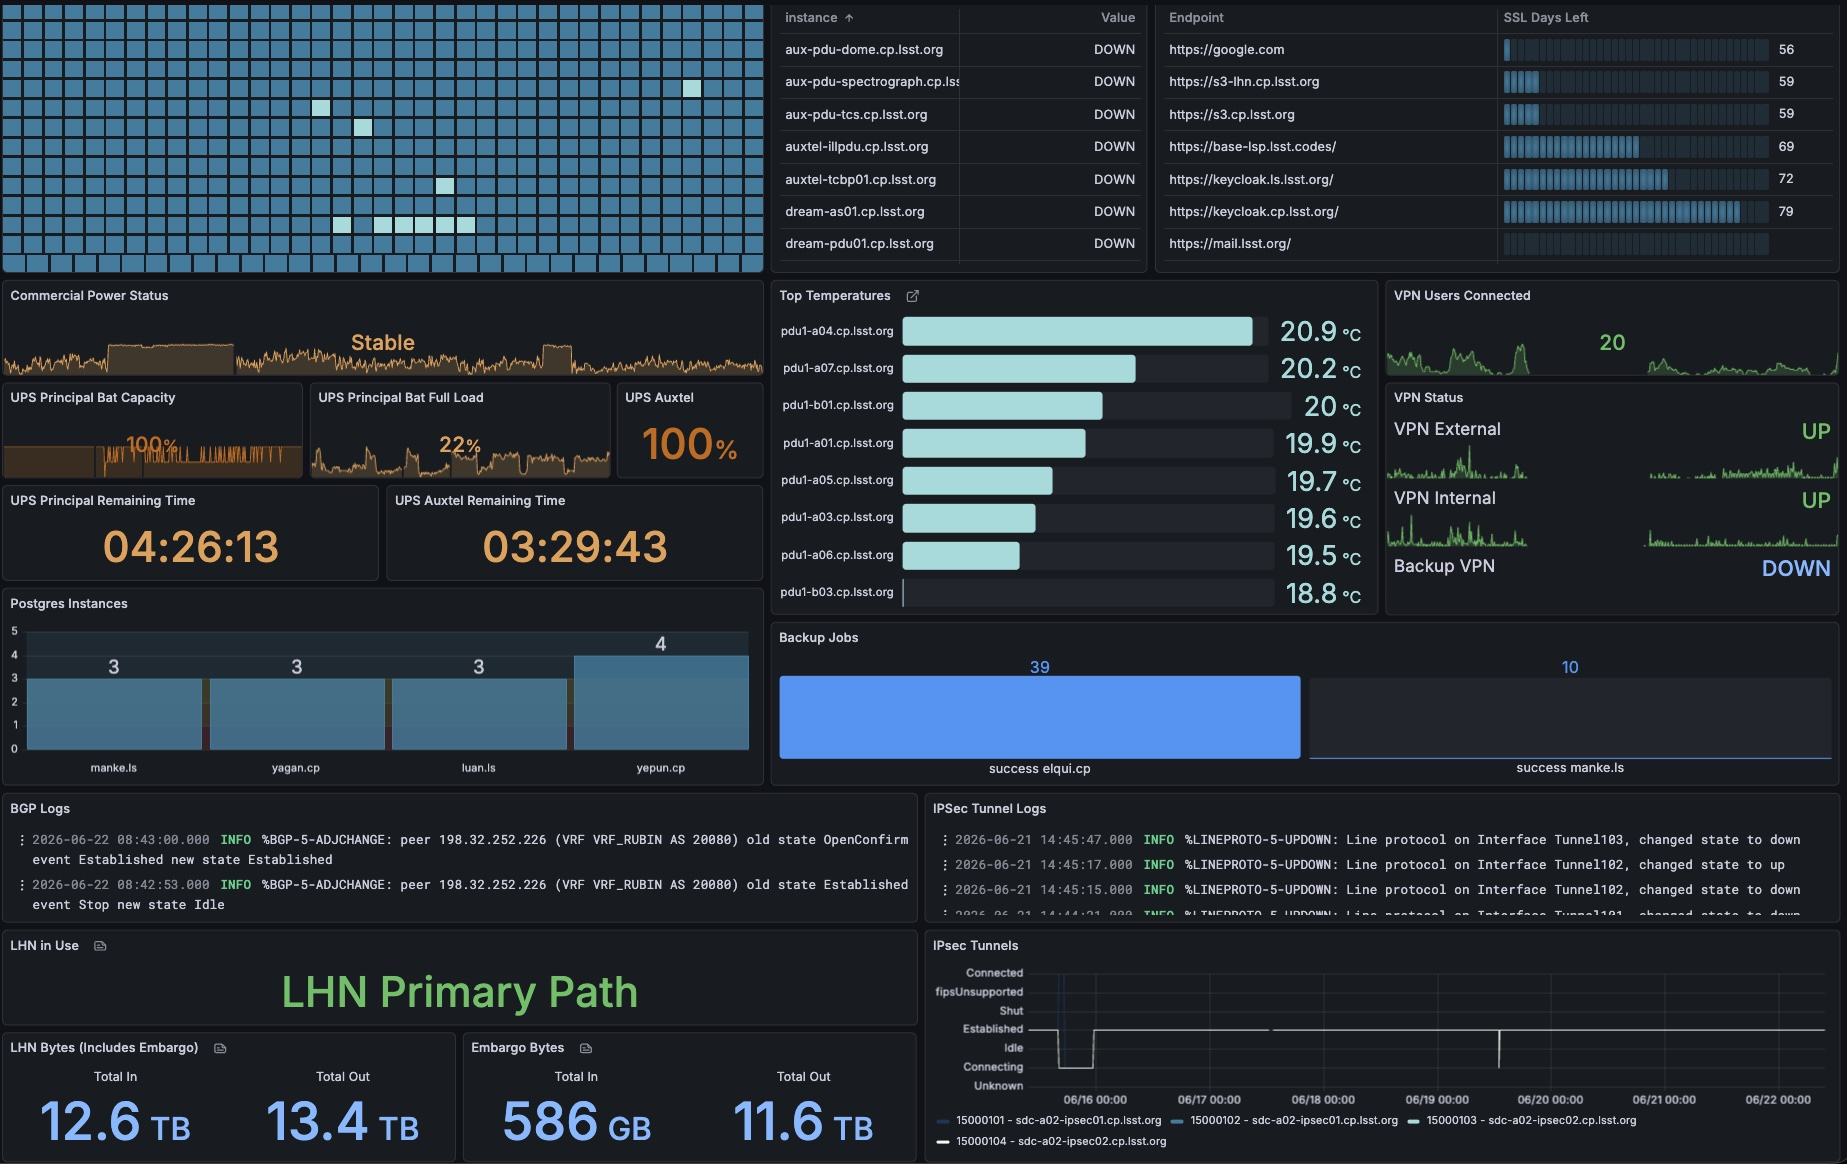
\includegraphics[width=\linewidth]{spie_dashboard.jpg}
        \\[4pt]
        \textbf{Figure 1.} Summary dashboard of several useful metrics for Engineers and Operators.
    \end{minipage}
\end{center}

One deliberate choice in the dashboard design is color. Every palette used across the dashboards
was selected to be readable under all common forms of color blindness \cite{wcag-color}. This is
not a cosmetic detail; it is an operational requirement. It does not matter how much information a
dashboard contains if the person looking at it cannot immediately tell that something is wrong, or
cannot distinguish between two states at a glance. Any engineer, operator, or scientist at the
observatory should be able to look at a panel and read it correctly, regardless of how they
perceive color.

The difference becomes clear when you simulate how the same dashboard looks under different visual
conditions. Under deuteranopia and protanopia, the two most common forms of red-green color
blindness, the conventional red/green palette collapses \cite{wcag-color}. Red and green become
nearly identical shades of brownish yellow. An operator glancing at the panel during a busy night
has no quick visual cue; they have to stop and read the label to know whether something is up or
down. That extra second matters when you are watching twenty panels at once.

\begin{center}
    \begin{minipage}{0.7\linewidth}
        \centering
        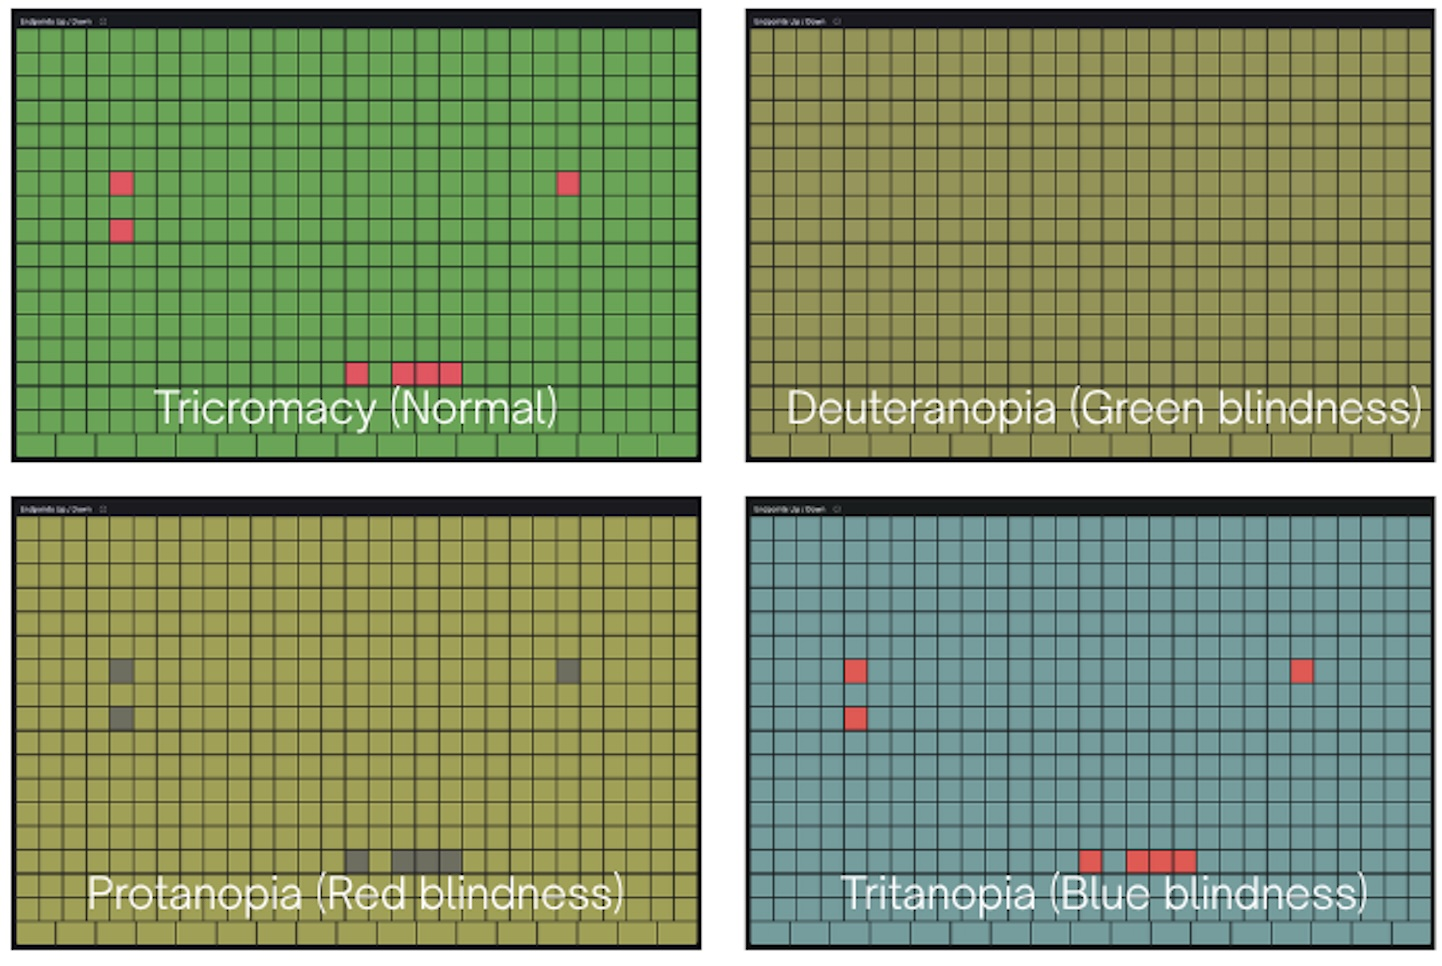
\includegraphics[width=\linewidth]{spie_red.jpg}
        \\[4pt]
        \textbf{Figure 2.} Up and Down monitor using default red and green colors, under different forms of color blindness.
    \end{minipage}
\end{center}

With our palette, the same simulation tells a different story. The colors remain visually distinct
under all tested conditions. The contrast is preserved not only in typical vision but also in
deuteranopia, protanopia, and tritanopia. Someone who has never been able to rely on red and green
to mean anything receives the same immediate signal as everyone else.

\begin{center}
    \begin{minipage}{0.7\linewidth}
        \centering
        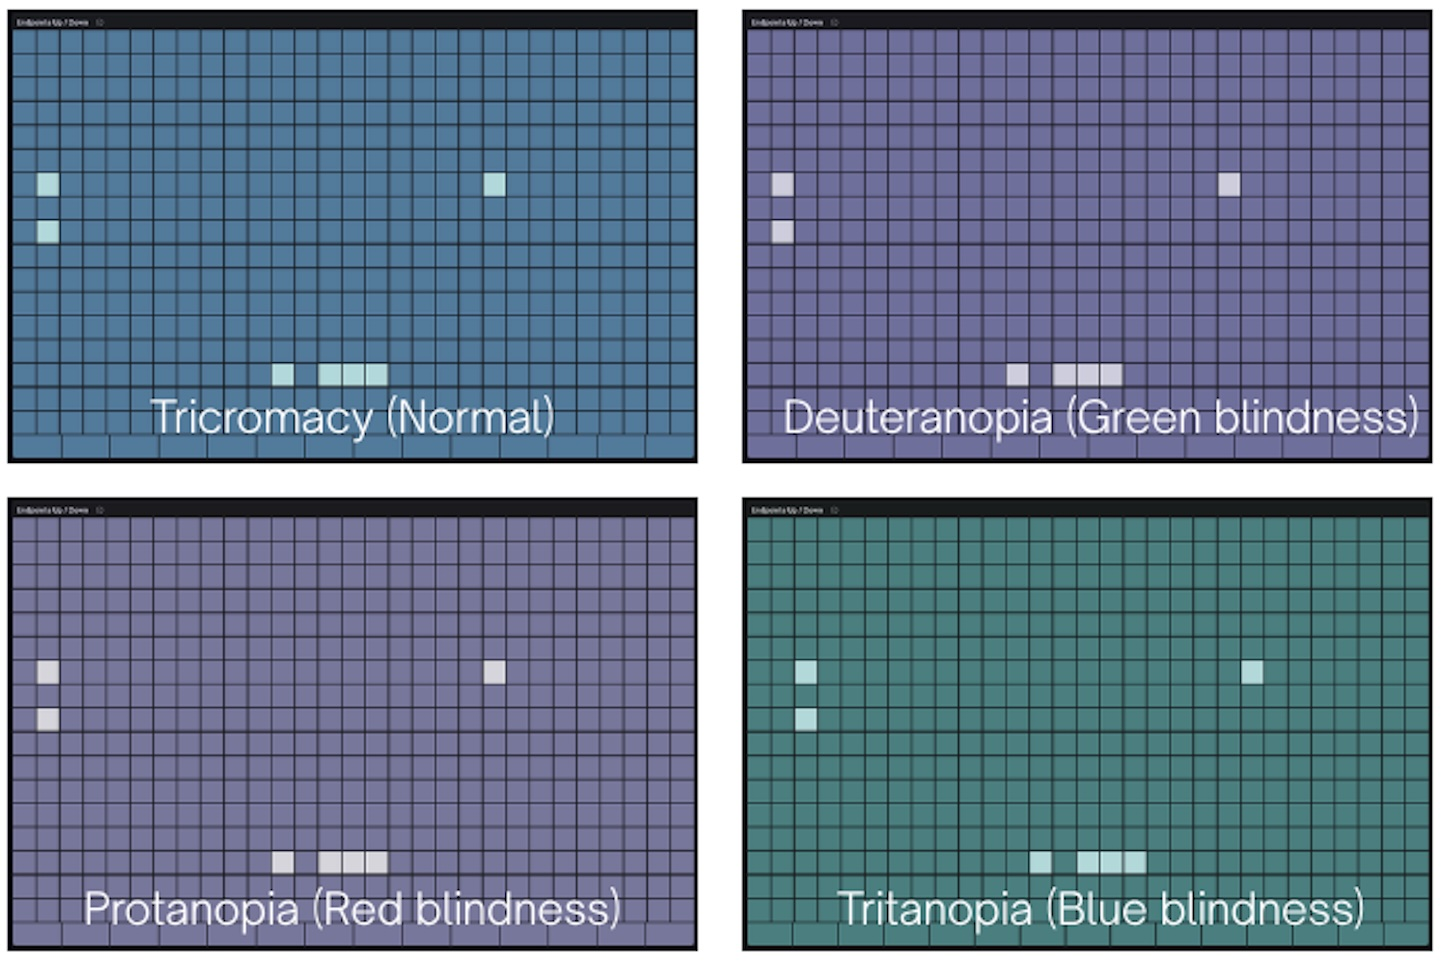
\includegraphics[width=\linewidth]{spie_nored.jpg}
        \\[4pt]
        \textbf{Figure 3.} Up and Down monitor using colors that can be noticeable under different forms of color blindness.
    \end{minipage}
\end{center}

That is the actual goal: not a palette that looks good in a screenshot, but one that works for
every person standing in front of the screens when it matters.

While this development only works with Rubin dashboards, we are exploring how to contribute this
work upstream so it can benefit the broader Grafana community.

\subsection{Alerting}

Alerts are a part of observability that interrupts people. That makes them different from
dashboards---a bad dashboard is inconvenient, but a bad alert wakes someone up at 3\,am for the
wrong reason, or worse, stays silent when something actually needs attention.

The platform stores alert rules as code, following the same review and promotion process as
everything else \cite{lsst-it-k8s-cookbook,prometheus-alerting,prometheus-alertmanager}. But the
technical side is the easier part. The harder part is writing alerts that are actually useful.

A good alert is not just a PromQL expression that fires when a number crosses a threshold
\cite{prometheus-alerting,prometheus-alertmanager}. It carries enough context to start a diagnosis:
what the condition is, how urgent it is, who should receive it, and where to look first. Without
that, an alert becomes noise, something that fires, gets acknowledged, and gets ignored. With it,
an alert is the first step of a structured response.

There is also a timing problem specific to night operations. During an observing shift, not
everything that is wrong needs immediate human attention. A saturated disk, a failed exporter, a
flapping network link, and a degraded storage component are serious, but they are not all the same
kind of serious. The alerting system needs to reflect that, routing the right signal to the right
person at the right time \cite{prometheus-alertmanager}, without flooding the on-call operator with
everything at once. Getting that routing right is ongoing work, and it improves the same way
everything else does: through real incidents, honest postmortems, and small adjustments that
accumulate over time.

\subsection{Discovery}

One of the quieter but more important parts of the platform is how it finds hosts to monitor.
There is no hand-maintained list. Instead, the platform queries the Puppet instances that manage
the observatory's infrastructure. Every time a new host is provisioned through the
infrastructure-as-code process, it becomes visible to the observability platform automatically, no
code changes, no manual additions, no tickets to update a configuration file.

This matters more than it might seem. In an environment that is still growing and changing, a
static host list becomes wrong almost immediately. A node brought up for commissioning, a host
added for a new instrument, all of them appear in the platform on their own, because the source of
truth is the infrastructure itself, not a separate list that someone has to remember to keep
current.

Services follow a different path, using Kubernetes-native discovery through label conventions. But
for the physical and virtual hosts that make up the observatory network, the answer is automatic:
provision the host, and the platform finds it.

\begin{center}
  \begin{minipage}{0.5\linewidth}
      \centering
      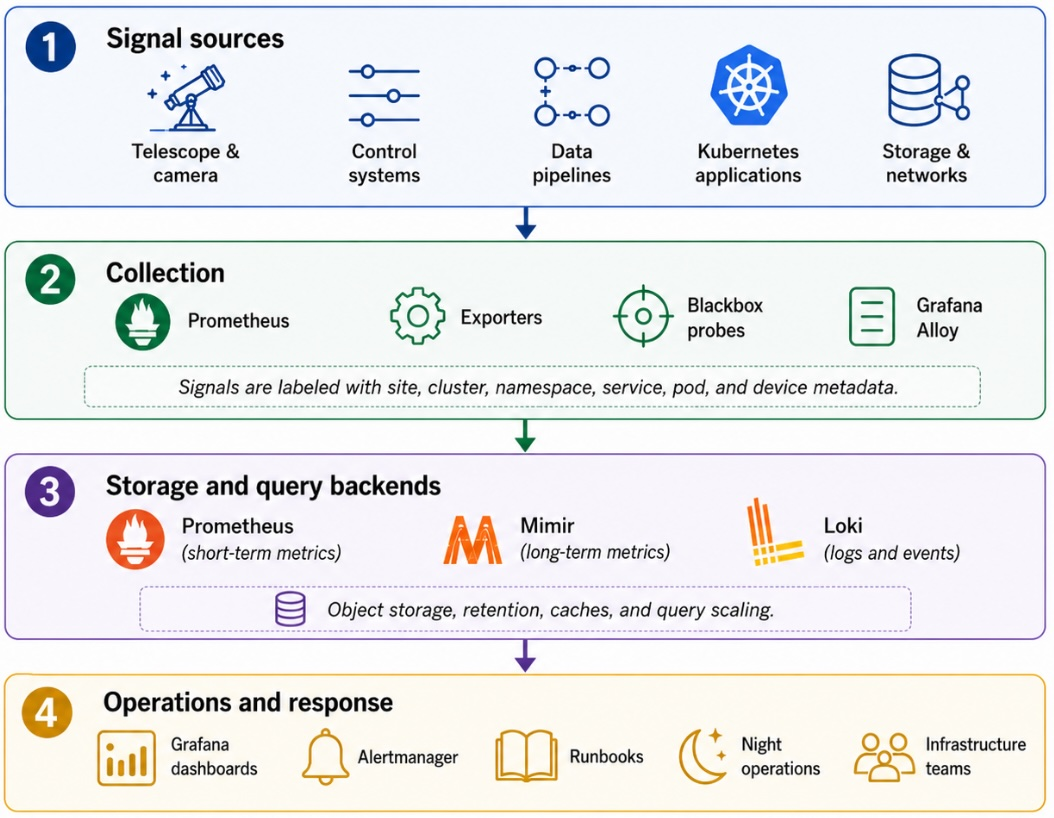
\includegraphics[width=\linewidth]{spie_arch.jpg}
      \\[4pt]
      \textbf{Figure 4.} Observability Architecture
  \end{minipage}
\end{center}% \textbf{TODO: ADD ARCHITECTURE DIAGRAM HERE}